\documentclass[a4paper,12pt]{article}

\usepackage[
    left=2cm,
    right=2cm,
    top=3cm,
    bottom=3cm
]{geometry}

\usepackage[utf8]{inputenc}
\usepackage[czech]{babel}
\usepackage[T1]{fontenc}
\usepackage{graphicx}
\usepackage{array}
\usepackage{booktabs}
\usepackage{tabularx}
\usepackage{makecell}
\usepackage{float}
\usepackage{newunicodechar}
\usepackage{url}
\usepackage{siunitx}
\usepackage{listings}
\usepackage{xcolor}
\usepackage{diagbox}
\usepackage{hyperref}
\usepackage{tikz}
\usepackage{pgfplots}
\pgfplotsset{compat=1.18}

\usepackage{fancyhdr}
\pagestyle{fancy}

\fancyhf{}
\fancyhead[L]{ARI -- Úkol 0: Opakování z předmětu SSI}
\fancyhead[R]{Pavel Pernička}
\fancyfoot[C]{\thepage}

\fancypagestyle{firstpage}{
    \fancyhf{}
    \renewcommand{\headrulewidth}{0pt}
    \renewcommand{\footrulewidth}{0pt}
    \fancyfoot[C]{\thepage}
}

\definecolor{myblue}{RGB}{111,0,248}
\newcommand{\colorcircle}[1]{%
  \tikz[baseline=-0.6ex]\draw[fill=#1,draw=none] (0,0) circle (1.5ex);%
}
\newcommand{\unitC}{\,^\circ\mathrm{C}}
\newcommand{\unitV}{\,\mathrm{V}}
\newcommand{\unitA}{\,\mathrm{A}}
\newcommand{\units}{\,\mathrm{s}}
\newcommand{\unitmin}{\,\mathrm{min}}

\newcommand{\centered}[1]{\begin{tabular}{l} #1 \end{tabular}}

\addto\captionsczech{\renewcommand{\refname}{Seznam použité literatury}}
\addto\captionsczech{\renewcommand{\figurename}{\textbf{Obrázek}}}
\addto\captionsczech{\renewcommand{\tablename}{\textbf{Tabulka}}}
\renewcommand{\lstlistingname}{\textbf{Kód}}

\lstset{
    language=Python,
    basicstyle=\ttfamily\footnotesize,
    keywordstyle=\color{blue},
    commentstyle=\color{gray},
    stringstyle=\color{red},
    numbers=left,
    numberstyle=\tiny\color{gray},
    stepnumber=1,
    breaklines=true,
    frame=single
}

\begin{document}
\thispagestyle{empty}

\vspace*{3cm}

\begin{center}


\includegraphics[width=0.35\textwidth]{img/ctu_logo.png}

\vspace{1.8cm}

{\Huge \textbf{ARI}} \\[0.6cm]

\rule{0.6\textwidth}{0.6pt} \\[0.8cm]

{\Large Úkol 0 -- Opakování z předmětu SSI}

\vspace{2.5cm}

{\large Pavel Pernička}

\vspace{0.3cm}

20.\,2.\,2026

\end{center}

\vfill

\newpage
\pagestyle{fancy}
\section{Úkol 1 -- Ustálená odezva}
\subsection{Statické zesílení}
Statické zesílení = DC gain. Ze zadání vidíme póly $s=-3$, $s=-2$, $S=-1$, pro všechny platí $\Re(s) < 0$, tedy jde o stabilní systém. Díky tomu můžeme určit DC gain jako:
$$
G(0) = \frac{5}{3\cdot 2\cdot 1} = \frac{5}{6}
$$

\subsection{Ustálená hodnota odezvy na vstup}
$$
W(s) = \frac{1}{s}\cdot G(s) = \frac{(-0,2s + 5)}{s\cdot (s+3)(s+2)(s+1)}
$$

$$
Y(s) = W(s)\cdot 5 = \frac{25-s}{s\cdot(s+3)(s+2)(s+1)}
$$

Z věty o koncové hodnotě:
$$
y(\infty) = lim_{s\to 0^+} sY(s) = \frac{25}{6}
$$

\subsection{Ustálená hodnota odezvy na dirracův impulz}
$u(t) = \delta(t)$, póly jsou nalevo, použijeme větu o koncové hodnotě:
$$
y(\infty) = lim_{s\to 0^+} s\cdot G(s) = lim_{s\to 0^+} \frac{s(-0,2s+5)}{(s+1)(s+2)(s+3)} = 0
$$

\section{Úkol 2 -- Laplaceova transformace}
\subsection{Řešení soustavy diferenciálních rovnic}
Na diferenciální rovnice aplikujeme Laplaceovu transformaci -- pro $x_1$:
$$
\mathcal{L}\left[\frac{d x_1}{dt}\right](s) = \mathcal{L}[-6x_1 + 26x_2](s)
$$

$$
X_1(s)\cdot s-2 = -6X_1(s) + 26 X_2(s)
$$

$$
X_1(s) = \frac{26 X_2(s) + 2}{s+6}
$$

pro $x_2$:
$$
\mathcal{L}\left[\frac{d x_2}{dt}\right](s) = \mathcal{L}[-\frac{1}{2}x_1](s)
$$

$$
X_2(s) = -\frac{X_1(s)}{2s}
$$

Nyní se vrátíme zpět do časové oblasti pomocí inverzní Laplaceovy transformace:
$$
x_1(t) = \mathcal{L}^{-1}[X_1(s)] = 2 e^{-3t} \cos(2t)\cdot 1(t) - 3e^{-3t}\cdot 1(t)
$$
$$
x_2(t) = \mathcal{L}^{-1}[X_2(s)] = -\frac{1}{2}e^{-3t}\cdot \sin(2t)\cdot 1(t)
$$

\subsection{Průběhy nalezených funkcí}
Průběhy z Matlabu jsou znázorněny na obrázku \ref{fig:x1}.
\begin{figure}[h]
  \centering
  
\includegraphics[width=0.8\textwidth]{img/ukol2_x1x2.pdf}
  \caption{Průběh funkcí $x_1(t)$ a $x_2(t)$ pro zadanou soustavu.}
  \label{fig:x1}
\end{figure}

\section{Úkol 3 -- Linearizace}
\subsection{Rovnovážný pracovní bod}
Hledáme rovnovážný pracovní bod $P = [x_{1p}\ x_{2p}\ y_p]$ pro $u_p(t) = 2$:
$$
0 = x_{2p}
$$
$$
0 = -2\sin(x_{1p})-\frac{1}{10}x_{2p}+u_p
$$
$$
\sin(x_{1p})=1 \Rightarrow x_{1p} = \frac{\pi}{2}+2k\pi
$$
$$
P = \left[\frac{\pi}{2}+2k\pi\ 0\ \frac{\pi}{2}+2k\pi\right]
$$

\subsection{Linearizace}
$$
\delta\dot{x_1} = \Delta x_2
$$
$$
\Delta\dot{x_2} = -2\cos(x_{1p})\Delta x_1-\frac{1}{10}\Delta x_2 + \Delta u = -\frac{1}{10}\Delta x_2 + \Delta u
$$
$$
\Delta y = \Delta x_1
$$
\subsection{Simulink}
(Nadaří se mi zprovoznit Simulink v Linuxové verzi Matlabu)

\section{Úkol 4 -- Asymptotické frekvenční charakteristiky}
\subsection{Obrázek charakteristiky}
\begin{figure}[h]
  \centering
  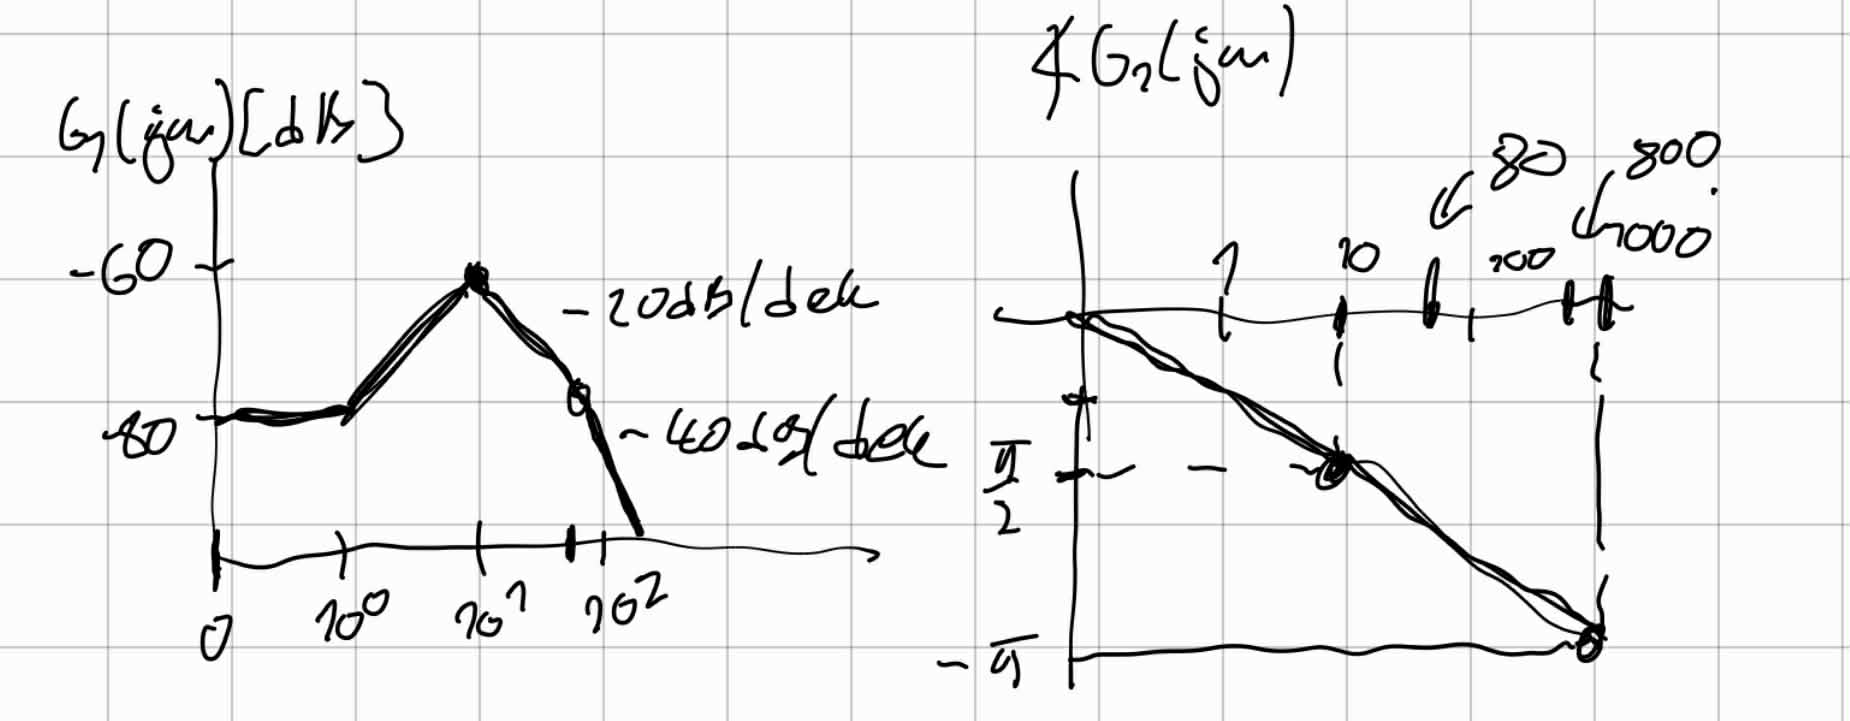
\includegraphics[width=0.8\textwidth]{img/ukol4.jpeg}
  \caption{Náčrt frekvenční charakteristiky $G_1(s)$}
  \label{fig:u4_nacrt}
\end{figure}

\subsection{Charakteristika z obrázku}
Z obrázku vidíme póly: $10^{-3}, 10^3$ a nuly: $10^{-1}, 10^1$. Z toho sestavíme:
$$
G_2(s) = K\cdot \frac{(1+10s)(1+0,1s)}{(1+10^3)(1+10^{-3}s)}
$$

Z fázové charakteristiky vidíme $K=-1$ a upřesníme znaménka:
$$
G_2(s) = -\frac{(1-10s)(1+0,1s)}{(1+10^3)(1+10^{-3}s)}
$$

\section{Úkol 5 -- Převod do přenosového popisu}
Chceme formát ($A,B,C,D$ jsou matice):
$$
\dot{x} = Ax + Bu
$$
$$
y = Cx
$$

Laplacujeme:
$$
sX(s) = BU(s)
$$
$$
Y(s) = CX(s)
$$

$$
X(s) = (s-A)^{-1} B\cdot U(s)
$$

$$
Y(s) = (C\cdot (s-A)^{-1}B+D)\cdot U
$$

$$
G(s) = \frac{Y(s)}{U(s)} = C\cdot (s-A){-1}\cdot B = \dots = \frac{4(s-3}{(s-2)(s+2)}
$$

\section{Úkol 6 -- Stabilita}
Stabilitu posuzujeme pomocí vlastních čísel systému, ty získáme z matice $A$: ${1, -1+i\sqrt{3}, -1-i\sqrt{3}}$. Vidíme, že $\Re(1) > 0$, systém je tedy nestabilní.

\section{Úkol 7 -- Diskretizace}
$G(s)$ má póly $s=-1$ a $s=-7$, odtud můžeme určit $T_{min} = \frac{1}{7}\ s$. Jako dobrou periodu volíme $T_1 = 0,05s$ a jako špatnou $T_2 = 0,5\ s$. Diskretizaci provádíme pomocí Matlabí funkce $c2d()$.
Průběhy jsou znázorněny na obrázcích \ref{fig:ukol7_T1} a \ref{fig:ukol7_T2}
\begin{figure}[H]
  \centering
  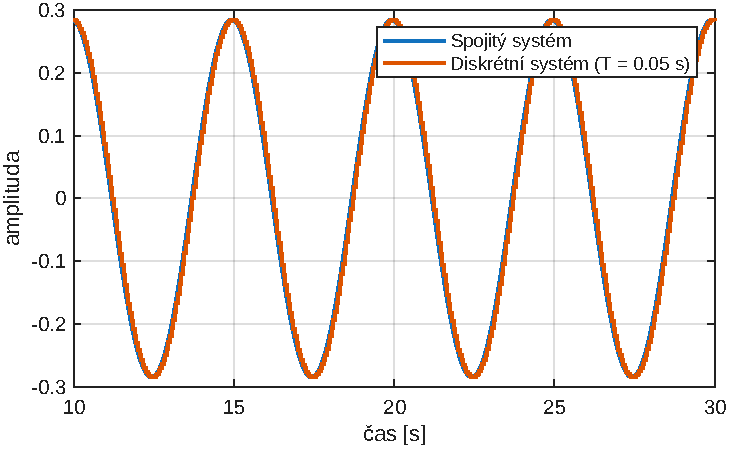
\includegraphics[width=0.8\textwidth]{img/ukol7_vhodna.pdf}
  \caption{Odezva spojitého a diskretizovaného systému pro vhodnou periodu vzorkování $T_1 = 0{,}05\,\mathrm{s}$.}
  \label{fig:ukol7_T1}
\end{figure}

\begin{figure}[H]
  \centering
  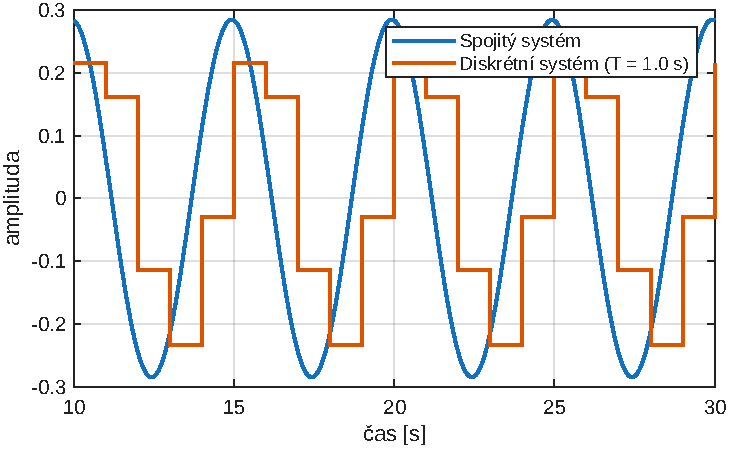
\includegraphics[width=0.8\textwidth]{img/ukol7_nevhodna.pdf}
  \caption{Odezva spojitého a diskretizovaného systému pro nevhodnou periodu vzorkování $T_2 = 0{,}5\,\mathrm{s}$.}
  \label{fig:ukol7_T2}
\end{figure}

\section{Úkol 8 -- Vlastnosti přenosů}
\begin{itemize}
    \item $\Re(s) < 0$ pro všechny póly $\Rightarrow$ stabilní, statický, nekmitavý
    \item póly $-\frac{1}{4}-\frac{\sqrt{17}}{4}$ a $-\frac{1}{4}+\frac{\sqrt{17}}{4}$ $\Rightarrow$ nestabilní, statický, nekmitavý
    \item dvojný pól v nule $\Rightarrow$ nestabilní, astatický, nekmitavý
    \item póly $-\sqrt{2}$ a $\sqrt{2}$ $\Rightarrow$ nestabilní, statický, nekmitavý
\end{itemize}

\section{Úkol 9 -- Spojování dynamických systémů}
\subsection{Paralelní zapojení}
$$
H(s) = G_1(s)+G_2(s) = \frac{s^2+1}{s(s+1)}
$$

\subsection{Sériové zapojení}
$$
H(s) = G_1(s)\cdot G_2(s) = \frac{s-1}{s(s+1)}
$$

\subsection{Zapojení podle obrázku 3}
$$
H(s) = \frac{Y(s)}{R(s)} = \frac{G_1(s)\cdot G_2(s)}{1+G_1(s) G_2(s)} = \frac{s-1}{s^2 + 2s -1}
$$

\subsection{Zapojení podle obrázku 4}
$$
Y(s) = X(s) G_1(s)
$$

$$
X(s) = R(s)-G_2(s)\cdot Y(s)
$$

$$
H(s) = \frac{Y(s)}{R(s)} = \frac{G_1(s)}{1+G_1(s) G_2(s)} = \frac{s(s-1)}{s^2 + 2s -1}
$$

\section{Úkol 10 -- Diskrétní systém}
\subsection{Přenos systému}
Na diferenční rovnici aplikujeme Z-transformaci:
$$
3Y(z) - z^{-1} Y(z) + \frac{1}{2}z^{-2} Y(z) = z^{-1} U(z) - z^{-2} U(z)
$$

$$
H(z) = \frac{z-1}{3z^2-z+\frac{1}{2}}
$$

\subsection{Stabilita systému}
Z přenosu vidíme póly $\frac{1\pm i\sqrt{5}}{6}$. Ty leží uvnitř jednotkové kružnice, systém je tedy stabilní

\subsection{Simulinkové schéma}
(Nejede mi Simulink)

\section{Úkol 11 -- Skokové a impulzní charakteristiky}
\subsection{Přiřazení charakteristik}
Metodou kouknu se a vidím máme dvojice: \textit{a:f},  \textit{b:d}, \textit{c:e}

\subsection{Vztah mezi impulzní a skokovou charakteristikou}
Skoková charakteristika je časovým integrálem impulsní charakteristiky a impulsní charakteristika je časovou derivací skokové charakteristiky. V diskrétním světě jde o operace sumy a diference.

\section{Úkol 12 -- Frekvenční charakteristiky}
\subsection{Přiřazení}
Dvojice jsou: \textit{a:f}, \textit{b:d}, \textit{c:e}.

\subsection{Zesílení pro fázi $-45\ deg$ pro obrázek 5f}
Pro tuto fázi z grafu vyčteme fázi $-3\ dB$.

\end{document}
